%! Author = Yan Wittmann


\chapter{Tätigkeitsbeschreibung} \label{ch:wochenberichte-shortened}

Im Folgenden wird eine Beschreibung der Tätigkeiten über die Praktikumswochen gegeben.

% Einarbeitung in CVSS 4.0
\section{Woche 1 - Einarbeitung in CVSS 4.0} \label{sec:bericht-wo-1}

% Woche 1 (2023-09-04 bis 2023-09-08)

\lweekdaymarginpar{\weekdayMondayLong}

Mein erster Arbeitstag im Praktikums bei der {\metaeffekt} fiel mit dem Ende der Sommerpause des Unternehmens zusammen.
Da ich bereits seit einiger Zeit im Unternehmen arbeite und ich meine eigenständigen Aufgabenbereiche habe, war eine Einführung für mich nicht notwendig.
Bei {\metaeffekt} ist mein Aufgabenbereich als Entwickler ein automatisiertes Vulnerability Monitoring für unsere Kunden in der Programmiersprache Java zu implementieren und zu betreuen.
Ich verbrachte den Montag damit, einige während der Sommerpause aufgetretene Fehler in den Systemen von Kundenprojekten zu korrigieren und Gespräche mit Kollegen zu führen.

Ein näherkommendes Thema war die anstehende Veröffentlichung des CVSS 4.0-Standards, die für den 31.\ Oktober 2023\footnote{\url{https://www.first.org/cvss/v4-0/}} geplant war.
Zu den CVSS-Versionen 2.0 und 3.1 soll auch unser System CVSS 4.0-Vektoren berechnen können.
Mit Karsten Klein, meinem Chef und Betreuer für das Praktikum, habe ich zudem vereinbart, während meines Praxis-Semesters zusätzliche tägliche Meetings mit ihm abzuhalten.

\sweekdaymarginpar{\weekdayTuesdayLong}

Am Dienstag startete ich damit, die zu dem Zeitpunkt noch unfertige Dokumentation und Beispiele von CVSS 4.0 zu studieren.
In diesen wurde die offizielle Referenzimplementierung\footnote{\url{https://github.com/RedHatProductSecurity/cvss-v4-calculator}} referenziert, die später noch sehr nützlich werden würde.
Ich dokumentierte meine Erkenntnisse über die Gemeinsamkeiten und Unterschiede in unserem internen Confluence Wiki.

\sweekdaymarginpar{\weekdayWednesdayLong}

Am Mittwoch begann ich mit einem ersten Versuch einer Implementierung der CVSS 4.0-Berechnungen.
Wie ich bereits gestern vermutet hatte, ist die Berechnung bei 4.0 mathematisch deutlich komplexer, mit Hamming-Distanzen zwischen Vektoren und der Interpolation und Skalierung von mehrdimensionalen Räumen, versehen.
Dank der RedHat JavaScript-Implementierung konnte ich Mittwoch das Grundgerüst für meine Implementierung in Java vorbereiten.

\sweekdaymarginpar{\weekdayThursdayLong}

Donnerstag musste ich feststellen, dass die Referenzimplementierung und die Spezifikation voneinander abweichen, was bei einem unveröffentlichten Standard zwar verständlich, aber nicht hilfreich ist.
Ich meldete dieses Problem zusammen mit inhaltlichen Fragen in einem GitHub-Issue\footnote{\url{https://github.com/RedHatProductSecurity/cvss-v4-calculator/issues/32}} und begann den Rest des Tages bereits, die Implementierung zu schreiben.

\sweekdaymarginpar{\weekdayFridayLong}

Am Freitag erhielt ich bereits Antworten darauf:
Wie erwartet ist die online-Spezifikation nicht aktuell.
Den Rest des Tages konnte ich meine Implementierung so weit fertigstellen, dass ich sie durch einen Test-Datensatz tatsächlich bereits validieren konnte.
Als Nächstes wollte ich mein Verständnis von CVSS 4.0 verbessern, bevor ich die neue Version noch richtig in unsere Systeme integriert muss.

Leider hat den restlichen Tag eine \qt{OutOfMemoryError}-Exception in einem Kundenprojekt meine Zeit eingenommen, die auftrat, wenn eine zu große Menge an Daten verarbeitet wurde.
Ich konnte das Problem, dass während der Serialisierung in ein HTML-Dokument das interne Modell (damit auch der Speicherbedarf) kurzzeitig dupliziert wurde, jedoch schnell beheben.
Freitagmittag findet bei der {\metaeffekt} ein wöchentliches Meeting statt (\qt{Weekly}), hier berichtete ich über meine Erfahrungen mit der Implementierung von CVSS 4.0.
So beendete ich meine erste Praktikumswoche.


% Vertiefung in CVSS 4.0 und Korrelationsdaten
\section{Woche 2 - Vertiefung in CVSS 4.0 \headerand Korrelationsdaten} \label{sec:bericht-wo-2}

% Woche 2 (2023-09-11 bis 2023-09-15)

\lweekdaymarginpar{\weekdayMondayLong}

Ich verbrachte den Montag damit, die Spezifikation\footnote{\url{htthttps://www.first.org/cvss/v4.0/specification-document}},
die Entwicklungsgeschichte\footnote{\url{https://www.first.org/cvss/v4.0/user-guide\#New-Scoring-System-Development}}
und den Code im Kontext der Berechnung der Scores tiefergehender zu verstehen.
Den ersten Schritt mit den MacroVektoren hatte ich ein bereits gut verstanden, das Problem war eher der zweiten Schritt mit der Interpolation zwischen den einzelnen MacroVektoren.
Ich konnte selbst nach einem ganzen Tag an Recherche keine zufriedenstellende Erklärung finden, wie die Berechnung in diesem Schritt funktioniert.

\sweekdaymarginpar{\weekdayTuesdayShort, \weekdayWednesdayShort}

In Abwesenheit eines Kollegen übernahm ich Dienstag seine Aufgabe, die Pflege von sog. \qt{Korrelationsdaten} (siehe Kap. \ref{subsec:projektbericht-grundlagen-vulnerability-monitoring}).
Dazu konnte ich ein von mir entwickeltes Tool nutzen, das ich kurz vor meinem Praktikum als Web-UI über Spring Boot neu aufgesetzt hatte.

\sweekdaymarginpar{\weekdayThursdayLong}

Da die Implementierung und Integration von CVSS 4.0 bis Wochenende abgeschlossen sein musste, musste ich mich mit den folgenden verbleibenden Aufgaben intensiv beschäftigen:
Das Parsing der Vektoren aus verschiedenen Quellen/Formaten, das korrekte Verarbeiten der Berechnung von Scores und Modifizieren von Vektoren und das Anzeigen der Ergebnisse in unseren HTML- und PDF-Reports.
Da keine externe Datenquelle bisher CVSS 4.0 Vektoren bereitstellt, basierten einige meiner Annahmen über deren Formate auf Vermutungen, die später eventuell noch angepasst werden müssen.
Ich nutzte den Rest des Tages, um viele Code-Muster, die ich aus der Referenzimplementierung übernommen hatte, durch Refactoring-Operationen eleganter und objektorientierter zu gestalten und Code zu deduplizieren.
Am Ende des Tages stellte ich Pull Requests für die drei betroffenen Code-Projekte fertig.

\sweekdaymarginpar{\weekdayFridayLong}

Freitag widmete ich mich erneut dem Verständnis von CVSS 4.0.
Unter anderem berechnete ich manuell mehrfach auf unterschiedliche Weisen die drei Beispiele der MacroVektor-Interpolation aus der Spezifikation, was mein Verständnis erheblich verbesserte.

Das Weekly am Ende des Tages dehnte sich von einer auf fast zweieinhalb Stunden aus, da nicht nur ich, sondern auch einige Kollegen, diese Woche viel erreicht hatten.


% Excel-Limitierungen & Präsentationsvorbereitung
\section{Woche 3 - Excel-Limitierungen \headerand Präsentationsvorbereitung} \label{sec:bericht-wo-3}

% Woche 3 (2023-09-18 bis 2023-09-24)

\lweekdaymarginpar{\weekdayMondayLong}

Montag sollte ich unseren automatisierten CPE Matching-Algorithmus zwischen Hardware- und Software-Komponenten zu unterscheiden lassen, sodass Softwarekomponenten nicht mehr Hardware CPEs (und umgekehrt) zugeordnet werden würden.
Ob eine Komponente Hardware oder Software ist, wollten wir durch eine für die einzelnen Komponenten vergebbare definierte Liste an Kategorien ermöglichen.
Die Implementierung war recht simpel, doch der Detailgrad dieser Kategorien war jedoch bisher noch nicht geklärt.
Nach einiger Recherche habe ich drei Vorschläge für meinen Chef vorbereitet und wir konnten uns recht schnell auf einen einigen.
Eine davon deutliche abweichende Drittmeinung eines anderen Kollegen hat die Diskussion den gesamten restlichen Tag einnehmen lassen.
Ohne eine Lösung zu finden, vertagten wir die Diskussion.

\sweekdaymarginpar{\weekdayTuesdayShort\ - \weekdayThursdayShort}

Den Dienstag konnte ich eine lang-ersehnte Verbesserung der Excel-Serialisierung und Deserialisierung unserer Software-Inventare vornehmen.
Das Zeichenlimit von $32.767$\footnote{\url{https://support.microsoft.com/en-gb/office/excel-specifications-and-limits-1672b34d-7043-467e-8e27-269d656771c3}} Zeichen pro Excel-Zelle stellte uns vor Probleme, da unsere Daten oft dieses Limit überschreiten.
Aktuell gibt es einen Workaround, der die Daten bereits im Datenmodell in mehrere Spalten aufteilt, was gewisse Probleme hervorbringt.
Mit einer eleganteren Lösung, die die Datenaufteilung nicht schon im Datenmodell, sondern erst beim (De-)Serialisierungsprozess vornimmt habe ich, zusammen mit einem allgemeinen Styling-Modell für Excel-Dokumente, die alte Implementierung ersetzt.

\sweekdaymarginpar{\weekdayFridayLong}

Freitagmorgen wurde ich von meinem Chef überrascht:
Nächste Woche Dienstag und Mittwoch sollte mit ihm und einer Kollegin nach Erfurt auf das Treffen des Arbeitskreises OpenSource\footnote{\url{https://www.bitkom.org/Bitkom/Organisation/Gremien/Open-Source.html}} unter dem Thema \qt{Open-Source-Communities} und auf das darauf folgende Forum OpenSource\footnote{\url{https://www.bitkom.org/bfoss23}} der {\bitkom} gehen.
Der eigentliche überraschende Punkt war, dass ich bei dem Treffen des Arbeitskreises eine 25-Minütige Präsentation vor 30 Leuten, unter anderem von RedHat, Siemens, DB Systel und anderen großen Unternehmen, über die \qt{Identifikation und Bewertung von Schwachstellen mit Inhalten aus öffentlichen Quellen} halten sollte.

Ich nahm mir den restlichen Tag für die Vorbereitung darauf.
Trotz der Unterstützung meines Chefs bei der Themenauswahl und Strukturierung, war klar, dass die Zeit knapp werden würde.
Ich schaffte es, die Präsentationsfolien weitestgehend zu erstellen, mit dem Skript hatte ich jedoch gerade erst begonnen.

\sweekdaymarginpar{\weekdaySaturdayShort, \weekdaySundayShort}

Und so kam das erste Mal, dass ich an einem Wochenende für die {\metaeffekt} gearbeitet habe.
Das Wochenende verbrachte ich damit, ein 11-seitiges Skript für die Präsentation zu schreiben, die Folien weiter anzupassen und Punkte notiert zu notieren, die ich noch mit meinem Chef am Montag besprechen wollte.
Am Sonntagabend hatte ich ein ausführliches Skript fertiggestellt.


% AK OpenSource & OpenSource Forum Erfurt
\section{Woche 4 - AK OpenSource \headerand OpenSource Forum Erfurt} \label{sec:bericht-wo-4}

% Woche 4 (2023-09-25 bis 2023-09-29)

\lweekdaymarginpar{\weekdayMondayLong}

Montag besprach ich dann mit meinem Chef noch die letzten Unklarheiten.
Einen der Teile der Präsentation konnte ich an meinen Chef abgeben, da ich mich mit diesem einen Thema nicht sonderlich gut auskannte.
Den Rest des Tages nutzte ich lieber Zuhause im Home-Office, um die Präsentation in Ruhe üben und meine Reisetasche für die morgige Reise nach Erfurt packen zu können.

\sweekdaymarginpar{\weekdayTuesdayLong}

Der Dienstag begann früh mit unserer Reise mit dem ICE nach Erfurt, die mein Chef und ich für eine letzte Durchsprache nutzten.
Angekommen in Erfurt ging es direkt in den nahegelegenen Räumlichkeiten der DB Systel, wo es zunächst einleitende Worte und eine Vorstandswahl gab.
Im Anschluss daran war ich mit meiner Präsentation dran, bei der trotz anfänglicher Nervosität alles reibungslos verlief:
Ich brauchte mein Skript kaum und das Feedback war ausschließlich positiv, was mich sehr gefreut hat, denn ich wollte einen Mehrwert in diese Runde bringen.

Abends wurde vom {\bitkom} eine Stadtführung und ein gemeinsames Abendessen mit anderen Teilnehmern des OpenSource Forums organisiert, an welchen wir teilnahmen.
So konnten wir uns auch mit den anderen Teilnehmern austauschen.

\sweekdaymarginpar{\weekdayWednesdayLong}

Das OpenSource Forum der {\bitkom} bot eine entspannte Alternative zum vorherigen Tag, bei dem die Teilnehmer vielfältige Präsentationen verfolgen und sich untereinander auszutauschen konnten.
Besonders spannend waren die Einblicke in die Open-Source-Strategien großer Unternehmen wie SAP, Siemens und Mercedes.
Die Parallelen im Bezug auf die aktuellen Herausforderungen und Lösungsansätze für die Verwaltung von Schwachstellen und Lizenzen von Open-Source-Software in ihren Produkten und Projekten haben mich etwas überrascht und bestätigten die Relevanz unserer Arbeit.

\begin{figure}[htbp] % here, top, bottom, separate page
    \centering
    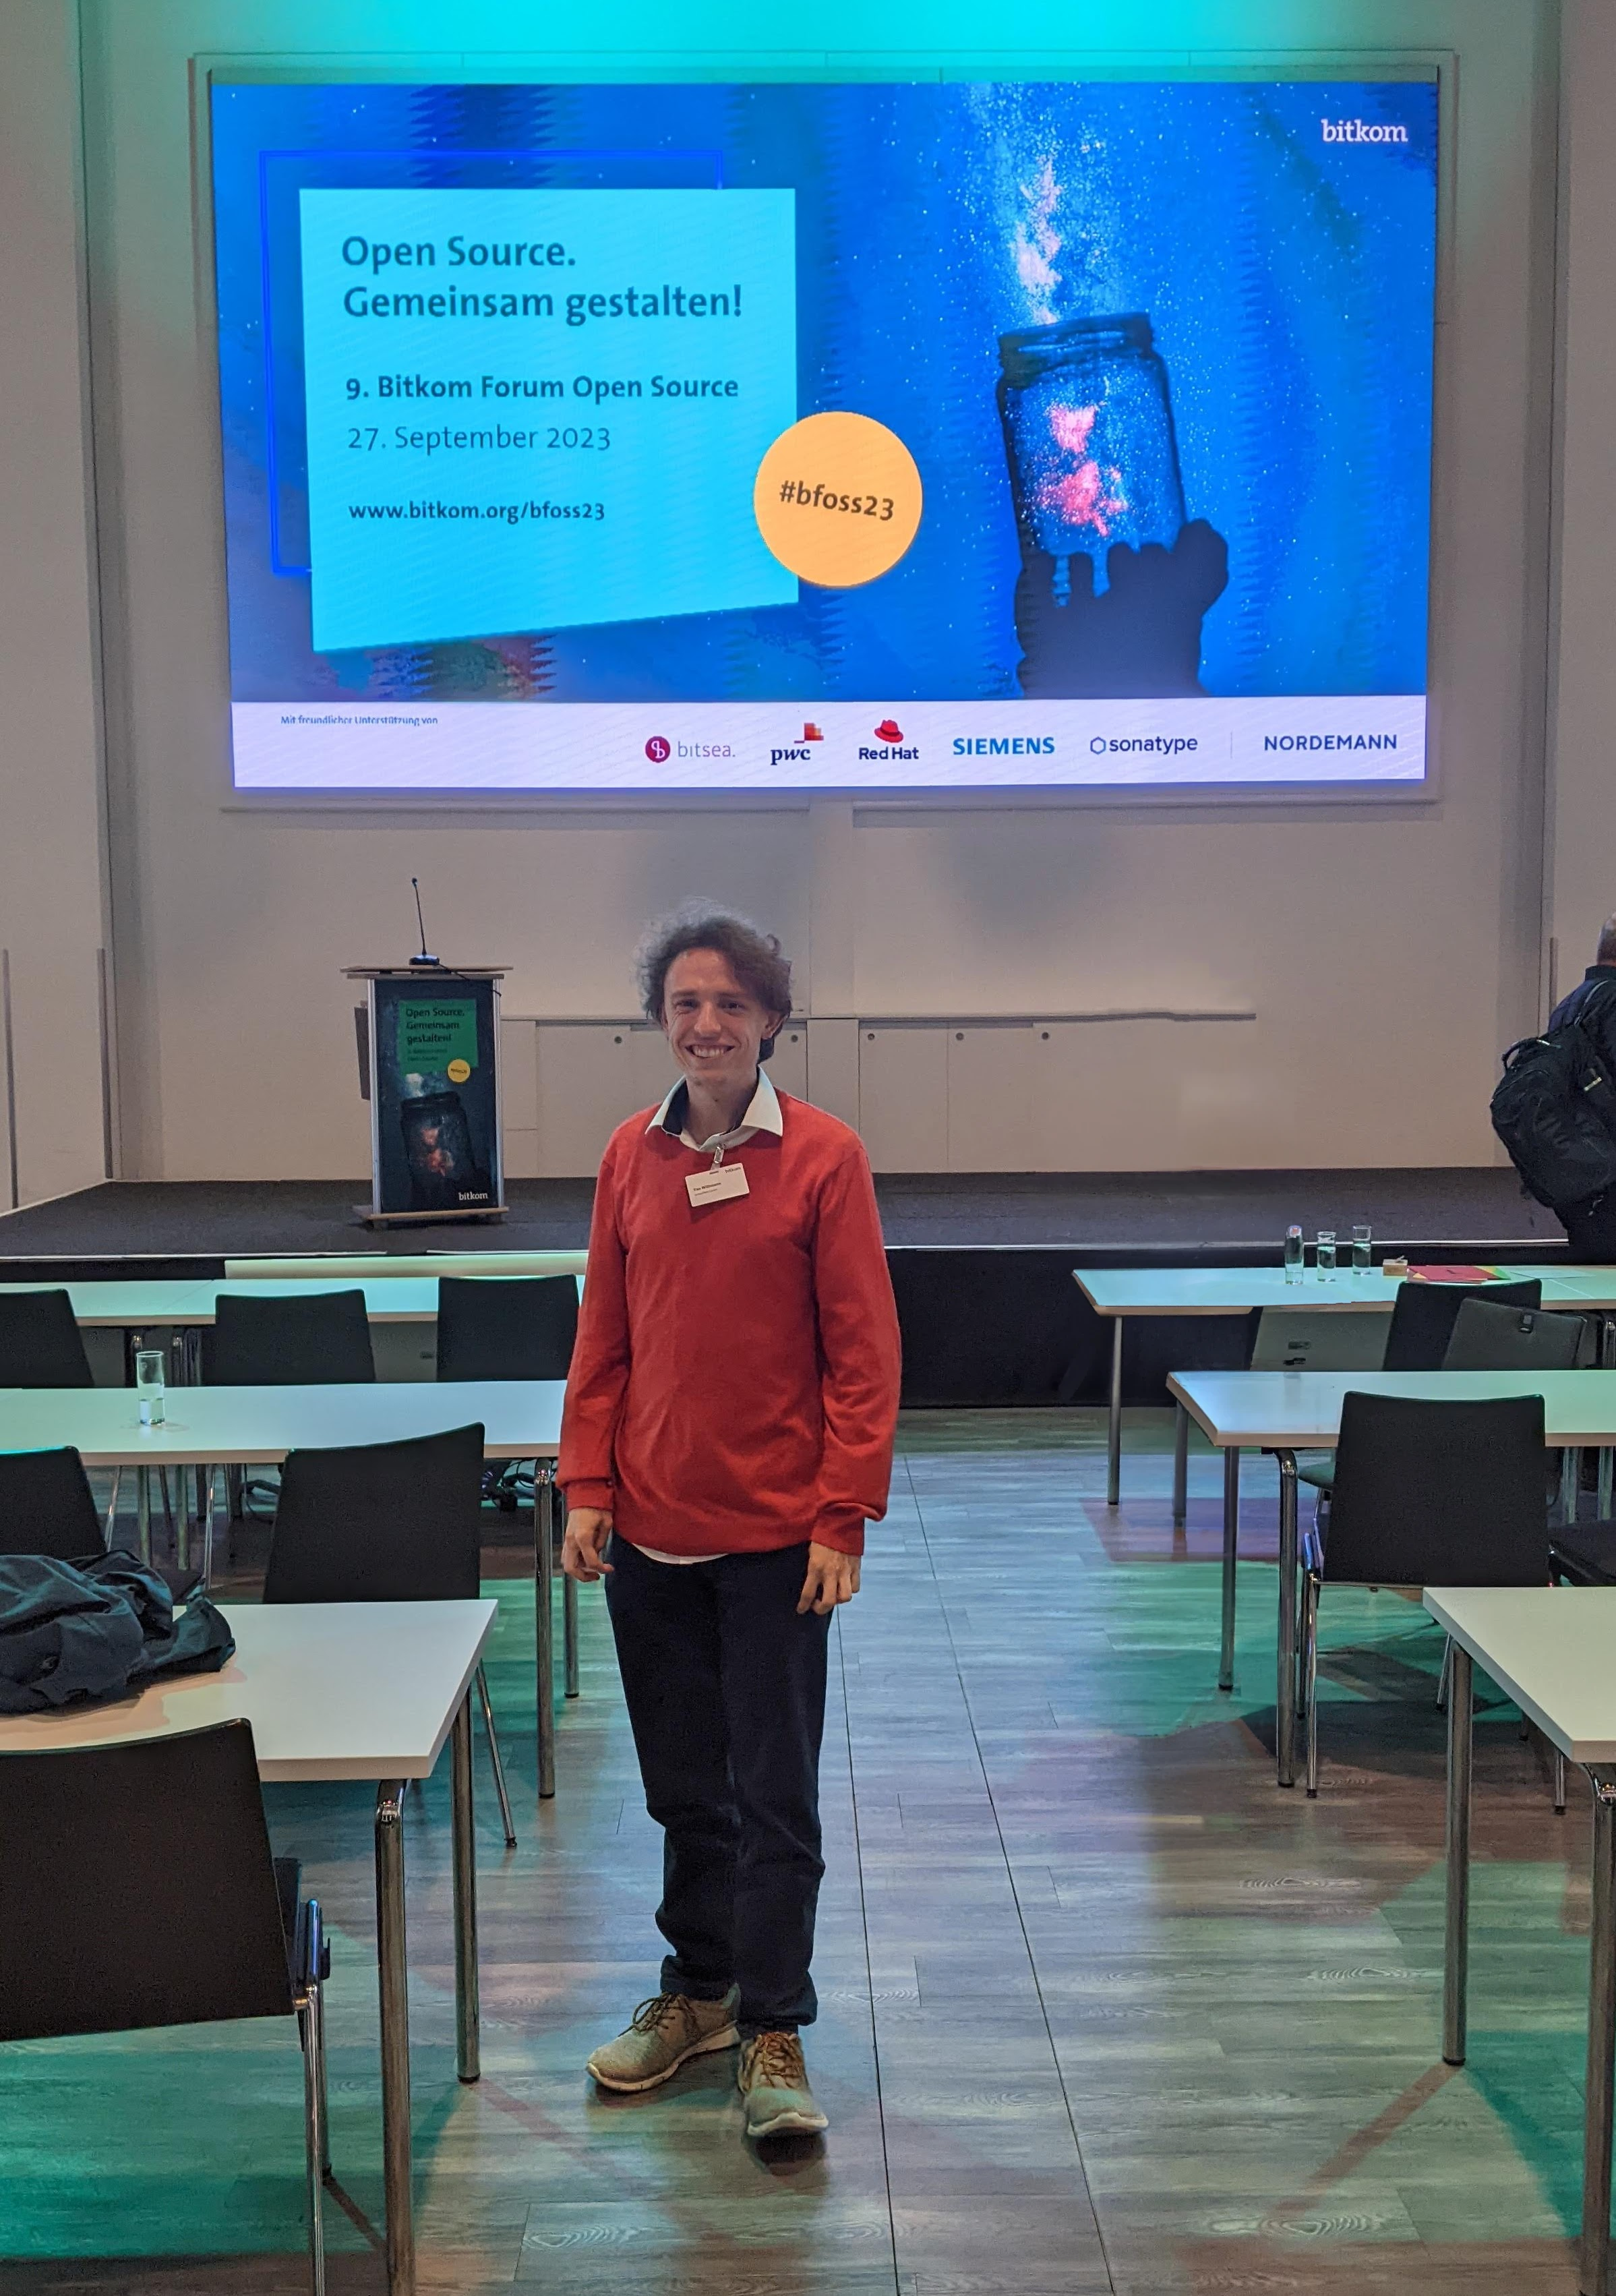
\includegraphics[width=0.5\textwidth, keepaspectratio]{res/img/2023-10-19-yan-ak-os}
    \caption{Auf dem Forum Open Source der Bitkom 2023}
    \label{fig:foss23-yan}
\end{figure}

Ein großer Programmpunkt war auch der {\bitkom} OpenSource Monitor\footnote{\url{https://www.bitkom.org/opensourcemonitor2023}}, der durch {\metaeffekt} gesponsert wird, wie in Abbildung \ref{fig:foss23-sponsor-metaeffekt} zu sehen ist.
Damit durfte die {\metaeffekt} einen Beitrag über den Cyber Resilience Act\footnote{\url{https://digital-strategy.ec.europa.eu/en/policies/cyber-resilience-act}} verfassen, der in diesem abgedruckt wurde.
Auch einige unserer direkten Kunden waren vertreten, die ich noch nie in Person getroffen hatte, außerdem konnte ich mit Studenten und Angestellten verschiedener Unternehmen sprechen.

\begin{figure}[htbp] % here, top, bottom, separate page
    \centering
    \includegraphics[width=0.8\textwidth, keepaspectratio]{res/img/2023-10-19-ak-os-metaeffekt-sponsor}
    \caption{Die {\metaeffekt} ist links als Sponsor zum OpenSource Monitor aufgeführt}
    \label{fig:foss23-sponsor-metaeffekt}
\end{figure}

\sweekdaymarginpar{\weekdayThursdayShort, \weekdayFridayShort}

Die Rückreise am Donnerstag verlief ohne Zwischenfälle, sodass der Freitag wieder der gewöhnliche Arbeitsalltag war.
Eine neue Kundenanforderung erforderte schon wieder direkte Aufmerksamkeit:
Einer unserer Download-Prozesse scheitert in ihrer Konfiguration, da der verwendete git-Befehl die konfigurierte Proxy-Informationen bislang scheinbar ignoriert.
Um das zu lösen, kann Git sowohl über einen Konfigurationsparameter im Befehlsaufruf, als auch über Umgebungsvariablen der Session konfiguriert werden.
Ich habe mich für die zweite Variante entschieden.

Ein persönliches Highlight war diesen Freitag allerdings, dass mein Bruder ab nächster Woche auch Teil des {\metaeffekt} Teams sein wird.


% Einarbeitung neuer Kollege (Nils)
\section{Woche 5 - Einarbeitung eines neuen Kollegen} \label{sec:bericht-wo-5}

% Woche 5 (2023-10-04 bis 2023-10-06)

\lweekdaymarginpar{\weekdayWednesdayLong}

Da Dienstag ein Feiertag war und ich montags einen Brückentag genommen hatte, war der Mittwoch mein erster Arbeitstag.
Die Einarbeitung meines neuen Kollegen war meine Hauptaufgabe für diese Woche.
Die Korrelationsdaten zu pflegen, also die Mappings zwischen unserer internen Darstellung von Software-Produkten und den Produkten in diversen externen Datenbanken, ist ab sofort sein Aufgabenbereich.
Passend dazu hat mein Chef uns einen neuen Datensatz gegeben, ein Inventar an Komponenten, den man einpflegen musste, anhand dem ich mit ihm die einfacheren Fälle und Grundlagen davon durchzugehen.

\sweekdaymarginpar{\weekdayThursdayLong}

Donnerstag habe ich erneut die etwas komplizierteren Fälle übernommen und ihn mit einigen einsteigerfreundlicheren versorgt.
Die Herausforderung für ihn als nicht-Informatiker an dieser Arbeit ist nicht nur die Methodik, sondern auch das gesammelte Wissen, das man über alle Software-Ökosysteme, Betriebssysteme und Software-Pakete haben muss.

\sweekdaymarginpar{\weekdayFridayLong}

Freitag habe ich ihm bereits etwas interessantere Fälle geben können und natürlich bei Fragen geholfen.
Ich bin etwas früher als er nach dem Weekly in das Wochenende gegangen.


% Weiter Daten-Korrelation & PowerShell Skripte
\section{Woche 6 - Daten-Korrelation \headerand PowerShell Skripte} \label{sec:bericht-wo-6}

% Woche 6 (2023-10-09 bis 2023-10-13)

\lweekdaymarginpar{\weekdayMondayShort\ - \weekdayWednesdayShort}

Da mein Kollege nicht das gesamte Inventar den Rest der Woche fertig bekommen würde, spielte sich diese Woche ähnlich wie letzte ab, in der ich meinen Kollegen bei der Arbeit unterstützte.
So konnte ich das Tool, das ich für diese Arbeit vor meinem Praktikum geschrieben hatte, selbst einmal anwenden und entdeckte einige Verbesserungsmöglichkeiten, die ich gleich umsetzte.
Das Tool (\qt{Correlation Utilities}) selbst ist Webapplikation, die mit einem lokal gehosteten Server, in Spring Boot implementiert, interagiert.
Das Ziel des Tools ist es, den Prozess des Mappings von unseren internen Produkten zu denen externer Datenbanken zu unterstützen.
Es aggregiert relevante Informationen automatisiert und macht Empfehlungen, wie am besten mit Fällen umgegangen werden sollte.
Dank des Tools besteht nun bereits fast keine Notwendigkeit, das ursprungs-Inventar zu durchsuchen oder Internet-Suchen zu starten.
Über die drei Tage habe ich es mit einigen weiteren Features erweitert.
Bis Mittwochabend hatten wir die Hälfte der Daten durchgearbeitet, den Rest sollte mein Kollege bis zum Ende der nächsten Woche erledigen.

\sweekdaymarginpar{\weekdayThursdayLong}

Donnerstag hatten mein Chef und ich morgens einen zweistündigen Termin mit einem unserer Kunden, {\aeclientZEZESE}, bei dem es um die automatisierte Erstellung einer SBOM (Software Bill of Materials) mit allen installierten Programmen, Treibern und Hardware-Devices auf Windows-Systemen ging.
Dieser Prozess sollte zweigeteilt sein:
Zunächst sollten über PowerShell-Skripte über Windows-Integrierte Features viele verschiedene Datenquellen angezapft und die rohen Ergebnisse in einem maschinenlesbaren Format in Dateien geschrieben werden.
Danach würde ein Maven-Plugin diese Daten analysieren und ein Inventar erzeugen.

Bis nächsten Montag sollten bereits erste Versionen der Skripte stehen.
Mein Arbeitslaptop selbst ist ein MacBook, also hat mir mein Chef einen zusätzlichen Windows-Laptop zum Entwickeln zur Verfügung gestellt.
An diesem habe mich zunächst einmal darüber informiert, wie man am besten an Windows-Systeminformationen gelangen kann.
Diese ersten Erkenntnisse habe ich zunächst in unserem internen Confluence niedergeschrieben, wo ich auch sonst meine Dokumentation ablege.

\sweekdaymarginpar{\weekdayFridayLong}

Freitag habe mich schnell wieder an das Thema gesetzt und mit den Ergebnissen meiner gestrigen Recherche angefangen, erste Skripte zur Sammelung von registrierten Programmen aus dem Store oder über Installers, die PNP-Devices (\qt{Plug and Play}) und Treibern.
Ich konnte die Hälfte der Use-Cases noch an diesem Tag durch verschiedene Skripte abdecken.


% PowerShell Skripte, Windows-Inventar & Strategieworkshop
\section{Woche 7 - Windows-Inventar-Extraktion \headerand Strategieworkshop} \label{sec:bericht-wo-7}

% Woche 7 (2023-10-16 bis 2023-10-20)

\lweekdaymarginpar{\weekdayMondayShort, \weekdayTuesdayShort}

Montag habe ich eine erste version der PowerShell Skripte fertigstellen können, die alle Use-Cases abdeckt.
Im Meeting später am Tag mit den Mitarbeitern von {\aeclientZEZESE} wurden meine Datensammlungs-Skripte dann live auf dem Ziel-Windows-Gerät erfolgreich ausgeführt.
Diese Daten auszuwerten hat gezeigt, dass sie noch nicht reichen, um ein vollständiges Bild zu erhalten, was ich dann den restlichen Tag durch Modifikationen an den Skripten geändert habe.

\sweekdaymarginpar{\weekdayWednesdayShort, \weekdayThursdayShort}

Die Entwicklung eines Java-Prozesses zur Verarbeitung von JSON-Daten aus PowerShell-Befehlen für ein Inventar im Format von {\metaeffekt} machte es nötig, die Ergebnisse der vielen verschiedenen PowerShell-Befehle zu kombinieren.
Wie bei Microsoft-Datenquellen so oft liefern die unterschiedlichen Befehle teils überlappende, teils einzigartige Datensätze, die nur zusammengenommen ein volles Bild ergeben.
Besonders bei Systeminformationen und PNP-Geräten waren Daten aus mehreren Befehlen zu konsolidieren.
Das Ergebnis war dann am Donnerstagabend ein vorläufiges Inventar, das zur Besprechung mit dem Kunden am Freitag noch etwas händisch aufbereitet wurde.

\sweekdaymarginpar{\weekdayFridayLong}

Der Freitag war ein ereignisreicher Tag:
Die {\metaeffekt} hat einen Strategieworkshop gehalten, der das Vorgehen der nächsten 9--12 Monate angeben sollte.
An einem großen Tisch und auf mehreren großen Whiteboard-Blättern wurden Wünsche und Pflichten aufgeschrieben und diskutiert.
Zu den Strategiepunkten, bei denen ich beteiligt sein werde, gehören die CVSS:4.0-Implementierung, eine Implementierung der CVSS-Versionen in TypeScript und eine Neuentwicklung des internen Datenmodells.

Das Meeting war sehr, hilfreich für mich, da es einen klaren roten Faden für das Semester vorgegeben hat.
Den Mitarbeitern von {\aeclientZEZESE} haben wir im Anschluss die Ergebnisse der Windows-Scans gezeigt und darum gebeten, dass sie die aktualisierten Skripte erneut ausführen, damit wir die vollständigeren Daten zu einem besseren Inventar umwandeln können.


% Abschluss Windows-Extraktion & Beginn Überarbeitung des Datenformats
\section{Woche 8 - Abschluss Windows-Extraktion \headerand Beginn Überarbeitung des Datenformats} \label{sec:bericht-wo-8}

% Woche 8 (2023-10-23 bis 2023-10-27)

\lweekdaymarginpar{\weekdayMondayShort, \weekdayTuesdayShort}

Mit den neuen Daten vom Freitag konnte ich Montag die Erkennung von Treibern, PNP-Devices und optionalen Features und die Performance des umfangreicheren Dateisystem-Scans einiger Skripte verbessern.
Um Dienstag die Windows-Extraktion vorerst abzuschließen, habe ich den restlichen Tag noch die PowerShell-Skripte unter einer MIT-Lizenz auf GitHub veröffentlicht und ein Maven-Plugin für die Inventar-Extraktion in Java geschrieben.

\sweekdaymarginpar{\weekdayWednesdayShort, \weekdayThursdayShort}

Mittwoch konnte ich (endlich) mit der Neuimplementierung der Datenstruktur und Logik dahinter beginnen.
Die einzelnen Tasks, die damit einhergehen, würden mich also die nächsten Wochen beschäftigen.
Bevor ich tatsächlich etwas programmieren konnte, wollte ich meine geplanten Änderungen in unserem internen Wiki dokumentieren und planen:
Begonnen habe ich mit dem Einführen eines Systems, das eine Quelle und Version eines Vektors eindeutig angeben kann.
Details dazu können in Kapitel \ref{subsec:projektbericht-loesungsweg-cvss-source-management} gefunden werden.
Eine erste Implementierung dazu konnte ich bereits Donnerstag fertigstellen.

\sweekdaymarginpar{\weekdayFridayLong}

Freitag habe ich damit verbracht, einem Kollegen zu helfen, der Probleme mit einer Software-Bibliothek hatte, die wir seit geraumer Zeit einsetzen.
Das Problem ließ sich am Ende auf einen internen Cache der Bibliothek zurückführen, den wir den Betreuern der Bibliothek in einem Issue\footnote{\url{https://github.com/spdx/Spdx-Java-Library/issues/215}} mitteilten.
Dieses Issue wurde einige Tage später durch einen Pull Request (PR) von meinem Kollegen behoben.


% Überarbeitung des Datenformats
\section{Woche 9 - Überarbeitung des Datenformats} \label{sec:bericht-wo-9}

% Woche 9 (2023-10-30 bis 2023-11-03)

\lweekdaymarginpar{\weekdayMondayLong}

Diese Woche begann ich mit der Überarbeitung des Datenformats für Schwachstellen und Security Advisories.
Das bisherige Datenformat besteht im Wesentlichen aus einer \codendt{Map<List<Map<String, String>\!>\!>}, wobei die einzelnen Ebenen zwar tatsächliche Instanzen mit weiteren Attributen und Methoden sind, aber sich nicht um das domänenspezifische  Parsen der Werte kümmern.

Dies bedeutet, dass komplexe Attribute oft über mehrere Schlüssel in der innersten Map verteilt sind oder aus einem strukturierten JSON-Objekt als String abgelegt werden.
Ein Problem dabei ist, dass man das Format dieser einzelnen Schlüssel genau kennen und es bei jedem Lese- und Schreibzugriff korrekt implementieren muss.

Obwohl Hilfsmethoden dafür zwar vorhanden sind, müssen diese trotzdem erst dem Entwickler bekannt sein und auch konsequent genutzt werden.
Es entsteht ein zusätzlicher Komplexitätsaufwand bei jeder Aufgabe, den man lieber vermeiden möchte.

Darum habe ich Montag ein System entworfen, das sich als Wrapper um die Zugriffe auf diese Klassen legt und dabei automatisch das korrekte (De-)Kodieren der Daten beim Ein- und Auslesen verwendet.

\sweekdaymarginpar{\weekdayTuesdayShort, \weekdayThursdayShort, \weekdayFridayShort}

Die Implementierung ist in zwei Schritten geplant, für jedes unserer betroffenen Module (core, artifact analysis).
Den Rest dieser Woche konzentrierte ich mich auf die Umsetzung des geplanten Systems in Artifact Analysis.
Dies beinhaltete vor allem die Entwicklung von Wrapper-Klassen für die inneren \code{Map<String, String>} Strukturen, die dafür verantwortlich sind, die Map in eine Kollektion von in unserem Datenmodell vorkommenden Instanzen umzuwandeln.
Zusätzlich plante ich eine Verwaltungsklasse, die für die korrekte Initialisierung aller Wrapper-Instanzen zuständig ist, diese verwaltet und die Verbindungsbeziehungen zwischen ihnen modelliert.

Die Programmierung dieser Komponenten erfolgte \qt{blind}, da ich den Code aufgrund von Konflikten zwischen dem bestehenden und dem neuen Datenmodell nicht ausführen konnte.
Das bestehende Datenmodell ist tief in unserer Codebasis integriert und stand an mehreren Stellen in Konflikt mit den neuen Strukturen.

Daher musste ich warten, bis die Änderungen in Artifact Analysis umgesetzt waren, was Freitagnachmittag \textit{fast} der Fall war.
Allerdings zog sich das wöchentliche Meeting länger als erwartet hin, wodurch ich die Umstellung diese Woche nicht vollständig abschließen und testen konnte.


% Abschluss Überarbeitung des Datenformats und CVSS Implementierung Verschieben
\section{Woche 10 - Abschluss Überarbeitung des Datenformats \headerand CVSS Implementierung Refactoring} \label{sec:bericht-wo-10}

% Woche 10 (2023-11-06 bis 2023-11-10)

\lweekdaymarginpar{\weekdayMondayLong}

Den Montag habe also damit verbracht, die Änderungen am Datenmodell und die Integration in die Prozessschritte in Artifact Analysis mit dem letzten verbleibenden Prozessschritt, dem VAD, zu vervollständigen\@.
Da hier alle Daten aggregiert dargestellt werden, ist dies einer der komplizierteren Schritte.
Zuerst ging es nur darum, die alte Funktionalität mit dem neuen Modell wiederherzustellen, ohne die neuen Features, die dadurch ermöglicht werden.
Einige Stunden später konnte ich immerhin den Code wieder ausführen, allerdings traten einige erwartete Fehler auf, die ich den restlichen Tag bearbeitete.

\sweekdaymarginpar{\weekdayTuesdayLong}

Die nächsten Tage konnte ich mich auf das Verschieben der CVSS-Implementierungen aus Artifact Analysis nach Core, in ein separates Modul, kümmern.
Die Aggregation der mehreren CVSS-Vektor-Quellen war zwar abgeschlossen, nun musste allerdings noch ein Prozess entworfen werden, der die Auswahl effektiver Vektoren und das korrekte Kombinieren und Überlagern ermöglicht.
Mit der Auswahl effektiver Vektoren habe ich den gesamten Dienstag verbracht, doch mein initialer Ansatz war zu naiv gedacht, weswegen ich die folgenden Tage einen neuen Ansatz verfolgte.

\sweekdaymarginpar{\weekdayWednesdayShort, \weekdayThursdayShort}

Mit diesem neuen Ansatz habe ich mir etwas länger Zeit gelassen, mit einigen Schaubildern und Testfällen zur Unterstützung.
Donnerstagnachmittag war der CVSS-Selektor dann fertig - deutlich komplizierter als anfangs erhofft, aber er konnte alle relevanten Fälle abdecken.

\sweekdaymarginpar{\weekdayFridayLong}

Um die Selektor-Logik in die bisherigen Prozessschritte einfügen war eine Nutzer-Konfiguration nötig, in der diese definierbar sind.
Ich habe in unserer Codebasis bereits ein recht umfangreiches Konfigurationssystem gebaut, was ich sehr einfach auf diesen Anwendungsfall anpassen konnte.
Mit meinem Chef zusammen habe ich beschlossen, dieses Konfigurationsobjekt auf alle Attribute auszuweiten, die etwas mit Security zu tun haben.
Diese neue zentrale Stelle habe ich vor und nach dem Weekly begonnen, überall zu integrieren und die alten Konfigurationsparameter durch diese auszutauschen.


% Transferieren der Datenklassen nach Core
\section{Woche 11 - Transferieren der Datenklassen nach Core} \label{sec:bericht-wo-11}

% 2023-11-13 bis 2023-11-17

\lweekdaymarginpar{\weekdayMondayLong}

Ende letzter Woche hatte ich die CVSS-bezogenen Features implementiert und in den Anreicherungsprozess integriert, sodass das System nun CVSS-Vektoren von beliebigen Datenquellen aufnehmen und deren Quellen nachvollziehbar halten konnte.
Den Montag nutzte ich, um diese Vektoren und deren berechneten Scores im VAD auf eine angereicherte Art anzuzeigen, was erstaunlich gut funktionierte.

\sweekdaymarginpar{\weekdayTuesdayLong}

Dienstagmorgen besprach ich mit meinem Chef die Integration dieser Änderungen in den PDF-Report unseres Core-Projekts.
Wir entschieden uns dazu, vorläufig Teile der Klassen in das andere Projekt zu kopieren, um auch dort Zugriff auf die Parsing-Logik zu haben, was zwar nicht schön ist (Code-Duplizierung), aber für jetzt die einfachere Lösung ist.
Noch am Dienstag konnte ich die relevanten Klassen in das Core-Projekt übernehmen und testen, wobei ich eine Namenskonvention für die kopierten Klassen festlegte und jeweils deren ursprüngliche Herkunft vermerkte.

\sweekdaymarginpar{\weekdayWednesdayShort, \weekdayThursdayShort, \weekdayFridayShort}

Mittwoch und Donnerstag stellte sich heraus, dass der Austausch des Datenmodells hinter dem PDF-Report mit dem kopierten Datenmodell komplexer war als erwartet.
Ich musste einige Abschnitte im Datenmodell leider komplett neu implementieren.
Den Rest der Zeit konnte ich dann das aktualisierte Modell in den Report einbinden.

Wir verwenden Apache Velocity mit einem textbasierten Template-XML-Format, was die Integration des neuen Modells aus mehreren Gründen sehr zeitintensiv machte.
Bis Freitagmittag war die Migration des Reports noch nicht abgeschlossen, allerdings hat war am Nachmittag ein Meeting mit einer Mitarbeiterin von \aeclientZEZESE\ geplant, um die Nutzung unseres VADs und die Bewertung von Schwachstellen in ihren Systemen zu besprechen.
Als Vorbereitung erstellte ich eine HTML-Seite, die unsere verschiedenen öffentlichen JSON-Schema-Dateien dynamisch zusammenfasst.
Das Meeting verlief erfreulicherweise angenehm und war produktiv für beide Seiten.


% Integration des Datenmodells in PDF-Report
\section{Woche 12 - Integration des Datenmodells in PDF-Report} \label{sec:bericht-wo-12}

% 2023-11-20 bis 2023-11-24

\lweekdaymarginpar{\weekdayMondayLong}

Am Montag erweiterte ich das Tracking-System der Matching-Konfigurationen aus verschiedenen Quellen von Schwachstellen, um nicht nur die bisherigen \qt{CPE}-Informationen, sondern auch Versionsbereiche und sogar Quellen wie GitHub und Microsoft zu integrieren.
Diese Informationen konnte ich noch am noch Montag in das VAD visuell ansprechend integrieren, was mir die Einfachheit von Anpassungen am VAD im Vergleich zum PDF-Report noch einmal deutlich machte.

\sweekdaymarginpar{\weekdayTuesdayShort, \weekdayWednesdayShort, \weekdayThursdayShort}

Die folgenden Tage kehrte ich wieder zur Integration des Datenmodells in den PDF-Report zurück.
Für jedes der etwa 20 Velocity-Templates ist der Prozess recht ähnlich:
Das Überprüfen der alten Datenzugriffe, im neuen Modell nach einem entsprechenden Zugriff suchen oder das Implementierte von neue Methoden, wiederholen sich stets.
Diese Änderungen nahm ich entweder in den Adapterklassen oder direkt im Modell vor, was Änderungen sowohl in Core als auch in Artifact Analysis erforderte.
Um den Dita-Renderingprozess (PDF-Generation aus Dita-Files) nicht bei jedem Test starten zu müssen, nutzte ich \qt{OxygenXML} für eine Live-Preview, doch der Prozess ist noch immer ein langer geblieben.

\sweekdaymarginpar{\weekdayFridayLong}

Freitag begann mit der Anfrage meines Chefs, ob ich an einem Workshop zum CSAF-Standard\footnote{\url{https://web.archive.org/web/20240121120954/https://www.allianz-fuer-cybersicherheit.de/Webs/ACS/DE/Netzwerk-Formate/Veranstaltungen-und-Austausch/CSAFversum/CSAFversum_node.html}} (Common Security Advisory Framework) teilnehmen möchte, der vom BSI in München organisiert wird.
Nach einer kurzen Recherche stimmte ich zu, da die Integration von CSAF in unser System schon länger geplant ist und mich persönlich auf eine Reise nach München freue.
Den Rest des Tages musste ich aufgrund der Abwesenheit eines anderen Kollegen erneut Korrelationsdaten für ein dringendes Inventar anlegen, bevor ich ins Wochenende starten konnte.


% Fertigstellung der Integration des Datenmodells & Dokumentation
\section{Woche 13 - Fertigstellung der Integration des Datenmodells \headerand Dokumentation} \label{sec:bericht-wo-13}

% 2023-11-27 bis 2023-12-01

\lweekdaymarginpar{\weekdayMondayShort, \weekdayTuesdayShort}

Nach einer Pause am Wochenende und der intensiven Report-Arbeit letzte Woche, konnte ich eben die Integration des Datenmodells in den Report bis Dienstagabend fast vollständig abschließen.
Dies schließt auch die neuen Segmente in den Templates zur Erklärung der Herkunft einer Schwachstelle ein.

\sweekdaymarginpar{\weekdayWednesdayShort, \weekdayThursdayShort}

Die Arbeit am neuen Datenmodell und Report war nun fast fertiggestellt.
Es blieben nur noch die Übersichtsdiagramme mit Statistiken über die gefundenen Schwachstellen für VAD (mit ChartJs\footnote{\url{https://www.chartjs.org}}) und PDF-Report (mit JFreeChart\footnote{\url{https://www.jfree.org/jfreechart}}) übrig.
Nachdem ich einige Zeit mit Reverse-Engineering der existierenden Diagramme verwendet hatte, musste ich zuerst einmal für zukünftige Zugriffe dokumentieren, welche Datenquellen wie verarbeitet werden und habe mit meinem Chef einige sinnvolle und lang geplante Änderungen an diesem Datenmodell besprochen.
Bis Donnerstag konnte ich das Thema des Refactorings des Datenmodells dann tatsächlich abschließen.

\sweekdaymarginpar{\weekdayFridayLong}

Da später im Praktikum diese Änderungen auch bei den Kunden angewendet werden müssen, habe ich am Freitag aus Voraussicht einen \qt{Migrationsguide} im internen Wiki erstellt, der alle Änderungen zwischen der alten und der neuen Generation unseres Systems dokumentiert.
Dieser Guide umfasst Themen wie die Änderungen an der CVSS-Implementierung, dem Tracking der CVSS-Vektoren und Schwachstellen, das neue Datenmodell, die neuen Konfigurationsparameter, neue Namenskonventionen und das restliche geändertes Verhalten.
Im Weekly Meeting berichtete ich, dass der neue Prozess nahezu abgeschlossen ist.


% Neuer Kollege, automatische Korrelationsdaten & Validierung des neuen Prozesses
\section{Woche 14 - Neuer Kollege, automatische Korrelationsdaten \headerand Validierung des neuen Prozesses} \label{sec:bericht-wo-14}

% 2023-12-04 bis 2023-12-08

\lweekdaymarginpar{\weekdayMondayLong}

Der Montag war auch der erste Arbeitstag eines neuen Kollegen, der uns bei der Entwicklung einer CI-Pipeline und eines Testing-Frameworks unterstützen sollte.
Ich half ihm vormittags bei der Einrichtung seines Laptops und erklärte ihm unsere Codebasis.
Nachmittags widmete ich mich einem anderen Kollegen, um über seine Änderungen an den Korrelationsdaten zu gehen, was den Rest des Tages in Anspruch nahm.

\sweekdaymarginpar{\weekdayTuesdayLong}

Diese gestrige Session mit den Korrelationsdaten erinnerte mich an die Art und Weise, wie wir Java-Versionen mit diesem System erkennen und, dass es nur ein provisorisches System sein sollte.
Ich entwarf Dienstag also ein System, das automatisch Korrelations-Einträge für alle bekannten Java-Versionen generieren kann.
Nach drei erfolglosen Iterationen über dieses Problem fand ich dann eine akzeptable und funktionierende Lösung und stellte sie dem Kollegen und meinem Chef vor.


\sweekdaymarginpar{\weekdayWednesdayShort, \weekdayThursdayShort}

In den folgenden Tagen nahm ich einen Schritt zurück, um den Refactoring-Prozess des Datenmodells noch einmal zu überprüfen.
Ich stellte fest, dass ich zwei größere Klassen vergessen hatte zu überführen und korrigierte zudem noch einige Fehler, die im Vergleich zu Generation 2 zu (zu stark) abweichenden Ergebnissen führten.
Nach diesen Korrekturen waren die Ergebnisse verbessert, und ich konnte endlich meine Generation 3 des Vulnerability-Monitorings meinem Chef präsentieren und besprechen.

\sweekdaymarginpar{\weekdayFridayLong}

Der bevorstehende CSAF-Workshop nächste Woche rückte näher, darum widmete ich den Freitag der Recherche über CSAF, indem ich die Dokumentation und einige Beispiele ansah.
Meine Erkenntnisse fasste ich in einem neuen Wiki-Artikel zusammen, wurde jedoch durch kleinere Anfragen und das wöchentliche Meeting immer wieder unterbrochen.
Die Recherche würde ich in der nächsten Woche fortsetzen.


% CSAF-Workshop in München
\section{Woche 15 - CSAF-Workshop beim BSI} \label{sec:bericht-wo-15}

% 2023-12-11 bis 2023-12-15

\lweekdaymarginpar{\weekdayMondayShort\ - \weekdayWednesdayShort}

Die Woche begann ich mit der Recherche zu CSAF, wobei ich mit der offiziellen Dokumentation\footnote{\url{https://docs.oasis-open.org/csaf/csaf/v2.0/os/csaf-v2.0-os.html}} begann.
Den Großteil der Zeit habe ich mich mit den JSON-Strukturen, Rollen der Teilnehmer, dem Produkt-Matching und den anderen Konzepten, die hinter CSAF stehen, beschäftigt.
Mir fielen einige Unterschiede zu anderen Standards auf, wie zum Beispiel, dass CSAF nicht nur das Format der Security Advisories definiert, sondern auch deren Veröffentlichung, Bereitstellung, Aktualisierung und Verarbeitung durch Endnutzer.
Diese Erkenntnisse hielt ich in einem Wiki-Eintrag fest und bereitete mich Mittwoch auf die Reise vor.

\sweekdaymarginpar{\weekdayThursdayLong}

Donnerstagmorgen reiste ich früh um 5:45 mit dem ICE zum Information Security Hub (ISH) des BSI am Flughafen München, wo der Workshop stattfand (Abbildung \ref{fig:yan-ish-csaf-muenchen}).

\begin{figure}[htbp] % here, top, bottom, separate page
    \centering
    \includegraphics[width=0.4\textwidth, keepaspectratio]{res/img/2023-12-14-yan-vor-dem-ish-muenchen}
    \caption{Vor dem \qt{Information Security Hub} am Münchner Flughafen}
    \label{fig:yan-ish-csaf-muenchen}
\end{figure}

Vor dem Workshop nutzte ich die Gelegenheit, mich mit anderen Teilnehmern von Bosch und anderen Unternehmen auszutauschen.
Der Workshop selbst war eine Mischung aus theoretischen Präsentationen und praktischen Übungen.
Es ging um die Begriffe, Rollen und Abläufe, aber auch um das tatsächliche Einsetzen der bereitgestellten Tools, dem eigenen erstellen von Security Advisories und dem Veröffentlichen dieser.
Besonders interessant waren für mich die Diskussionen über die Produktidentifikation und dem CVSS-Standard.
Nach dem Workshop und weiteren Gesprächen am abschließenden Buffet beendete ich den Tag mit einem Telefonat mit meinem Chef.

\sweekdaymarginpar{\weekdayFridayLong}

Freitag setzte ich die Teilnahme am Workshop fort, heute war der Fokus auf der praktischen Anwendung des CSAF-Standards.
Ich konnte, nachdem ich die Aufgaben recht schnell abschließen konnte, anderen Teilnehmern dabei helfen, die weniger Informatiker sind als Planer und Manager.
Nach dem Workshop und abschließenden Gesprächen machte ich mich auf den Heimweg und kam sogar dank einer früheren Verbindung schneller nach Hause.
Meine ausführlichen Notizen und Überlegungen würde ich in der folgenden Woche präsentieren.


% Letzte Woche vor der Weihnachtszeit
\section{Woche 16 - Letzte Woche vor der Weihnachtszeit} \label{sec:bericht-wo-16}

% 2023-12-18 bis 2023-12-20

\lweekdaymarginpar{\weekdayMondayLong}

Im Gegensatz zum letzten Jahr, wo das Weihnachtsfest ins Neujahr zurückverschoben werden musste, fand das Weihnachtsfrühstück der \metaeffekt dieses Mal frühzeitig im Schwarzen Walfisch statt.
Nach diesem gemeinsamen Frühstück kehrten wir ins Büro zurück, wo ich einen kurzen Bericht über den CSAF-Workshop für unsere Website verfasste\footnote{\url{https://metaeffekt.com/\#news}} und mit dem neuen Kollegen ein Testkonzept für unseren Software-Scanner diskutierte.

\sweekdaymarginpar{\weekdayTuesdayShort, \weekdayWednesdayShort}

Die restlichen Tage vor dem Urlaub widmete ich mich dem Abschluss des Refactorings meines Datenmodells, einschließlich Dokumentation und Code-Aufräumarbeiten.
Nach einem ausführlichen Gespräch mit meinem Chef über den Workshop konnte ich den Pull Request für die dritte Generation unseres Vulnerability Monitoring Toolings fertigstellen.
Mittwochabend ging ich gemeinsam mit den Kollegen in die Weihnachtsferien.


% TypeScript CVSS Calculator
\section{Woche 17 - TypeScript CVSS Calculator} \label{sec:bericht-wo-17}

% 2024-01-08 bis 2024-01-12

\lweekdaymarginpar{\weekdayMondayLong}

Das neue Jahr begann mit der Aufgabe, einen CVSS-Rechner in TypeScript zu entwickeln, der dann in ein zu entwickelndes Web-Interface integriert werden soll.
Dieses Interface soll die Scores für beliebig viele Vektoren, unabhängig von ihrer Version, berechnen und visualisieren können.
Für das gesamte Projekt ist später eine Veröffentlichung unter einer Open-Source-Lizenz auf GitHub vorgesehen.
Am Montag richtete ich zunächst das Projekt auf unserem lokalen git-Server ein, bereitete einen Build-Prozess mit Webpack vor und legte leere Klassen und Interfaces an.

\sweekdaymarginpar{\weekdayTuesdayShort\ - \weekdayFridayShort}

Die restliche Woche übersetzte ich die Java-Implementierungen in TypeScript und nutzte Jest\footnote{\url{https://jestjs.io/}} für Tests.
Ich erstellte einen Datensatz von 20.000 Vektoren pro CVSS-Version mit ihren erwarteten Scores für automatisierte Tests, anhand denen ich die Implementierungen entwickelte.
Bis zum Ende der Woche hatte ich die Klassen für CVSS:2.0 und CVSS:3.0 fertiggestellt und begann Freitag noch mit der komplexeren Version CVSS:4.0, konnte sie aber noch lange nicht fertigstellen.


% CVSS Calculator Web UI
\section{Woche 18 - CVSS Calculator Web UI} \label{sec:bericht-wo-18}

% 2024-01-15 bis 2024-01-19

\lweekdaymarginpar{\weekdayMondayShort, \weekdayTuesdayShort}

Den Beginn der Woche verbrache ich damit, die Implementierung von CVSS:4.0 abzuschließen.
Im Vergleich zur offiziellen JavaScript-Referenzimplementierung\footnote{\url{https://github.com/RedHatProductSecurity/cvss-v4-calculator/blob/main/app.js}} ist mein Ansatz in TypeScript deutlich objektorientierter und meiner Meinung nach übersichtlicher.
Zum Übernehmen der Implementierung einen eher ungewöhnlichen Ansatz gewählt, ich übertrug die Java-Klassen erst einmal 1:1 in TypeScript und passte sie dann Stück für Stück an die andere Sprache an.
Zirkuläre Referenzen löste ich mit madge\footnote{\url{https://www.npmjs.com/package/madge}}, aber ansonsten verlief alles in Ordnung.

\sweekdaymarginpar{\weekdayWednesdayShort, \weekdayThursdayShort, \weekdayFridayShort}

Nachdem alle Tests bestanden waren, implementierte ich das Web-Interface mit Bootstrap\footnote{\url{https://getbootstrap.com/}} und ChartJs.
Ich erstellte eine HTML-Struktur und entsprechendes JavaScript, um mit der CVSS-Bibliothek oder der NVD-API zu interagieren.
Nach der Basisfunktionalität verbesserte ich das UI, fügte Lizenzinformationen hinzu, räumte die Bibliothek auf und erstellte Dokumentation.
Das Ergebnis kann in Abb. \ref{fig:metaeffekt-cvss-calculator-ui} gesehen werden.
Das Projekt veröffentlichte ich auf GitHub\footnote{\url{https://github.com/org-metaeffekt/metaeffekt-universal-cvss-calculator}} und teilte es auf LinkedIn\footnote{\url{https://www.linkedin.com/feed/update/urn:li:activity:7151175714694729728/}}.
Das Feedback von unseren Kunden war sehr positiv, mit vielen Verbesserungsvorschlägen.

\begin{figure}[htbp] % here, top, bottom, separate page
    \centering
    \includegraphics[width=0.8\textwidth, keepaspectratio]{res/img/metaeffekt-cvss-calculator-ui}
    \caption{Der {\metaeffekt} Universal CVSS-Rechner}
    \label{fig:metaeffekt-cvss-calculator-ui}
\end{figure}

Von Herrn Shane Coughlan (OpenChain General Manager und ein Referent vom Open Source Forum der bitkom) haben wir freundlicherweise folgendes Zitat zu unserem Rechner erhalten:

\begin{quote}
    \textit{\qt{Contextualizing security threats is as important as identifying their existence,” says Shane Coughlan, OpenChain General Manager. “The emergence of open source tools to visualize this is a key part of ensuring the supply chain can plan ahead and action responses. We are delighted to see the work by Metaeffekt, an official OpenChain Partner, in the domain. It aligns well with OpenChain ISO/IEC 18974, the international standard for open source security assurance.}}
\end{quote}


%
\section{Woche 19 - Assessment-Policy \headerand Generation 3 Fertigstellung} \label{sec:bericht-wo-19}

% 2024-01-22 bis 2024-01-26

\lweekdaymarginpar{\weekdayMondayShort\ - \weekdayWednesdayShort}

Für einen unserer Kunden, der in die nächste Projektphase ihres Schwachstellmanagements gehen und nun Bewertungen vergeben möchte, erstellte ich den Anfang der Woche eine Assessment-Policy als Grundlage für ihre eigene Policy.
Das 6-seitige Dokument behandelt den Prozess des Vulnerability Monitorings, kontextualisiertes Re-Scoring mit CVSS, die Bedeutung einzelner CVSS-Metriken, die Vergabe von Status, Risiken und Maßnahmen sowie die Priorisierung von Schwachstellen.

\sweekdaymarginpar{\weekdayThursdayLong}

Zusammen mit einer Kollegin habe ich dieses Dokument Donnerstag noch einmal überarbeitet und an meinen Chef übergeben, der es auch noch einmal überarbeitet und dann mit unseren Kunden durchgesprochen hat.

\sweekdaymarginpar{\weekdayFridayLong}

Um die Änderungen der Generation 3 des Vulnerability Monitoring noch vor den Workshops des Kunden anzuwenden, wurde Freitag der große Pull Request endlich gemerged.
Den restlichen Tag habe ich weitere Anpassungen am CVSS-Rechner aufgrund von Feedback vorgenommen.
Es war zudem ein alter Kollege zu Besuch, mit dem wir nach der Arbeit noch einige Zeit verbrachten.


%
\section{Woche 20 - BSI-Meeting \headerand Integration von Generation 3} \label{sec:bericht-wo-20}

% 2024-01-29 bis 2024-02-02

\lweekdaymarginpar{\weekdayMondayLong}

Montags fand mit dem BSI ein Meeting bezüglich des CSAF-Standards und unseres CVSS-Rechners statt, mit Thomas Schmidt\footnote{\url{https://www.it-meets-industry.de/de/referent-thomas-schmidt}}, welcher bereits Leiter des CSAF-Workshops in München Ende letzten Jahres war, und Herr Von Samson.
Nach einer Demo unseres Toolings konnten wir nicht nur zur CSAF-Integration, sondern auch zum CVSS-Rechner, einige Tasks ableiten.
Thomas Schmidt erstellte in den folgenden Tagen dazu noch einige Issues auf unserem GitHub-Repository.

\sweekdaymarginpar{\weekdayTuesdayShort, \weekdayWednesdayShort, \weekdayThursdayShort}

Die restliche Woche startete dann die Integration von Generation 3 unseres Monitorings bei den mehreren Projekten unserer Kunden, um alle einheitlich von Generation 1 und 2 auf die neueste Generation 3 zu heben.
Der Prozess beinhaltete die Aktualisierung der Versionen und vor allem der Konfigurationen zum neuen Format, wobei der zuvor verfasste Migrationsguide wirklich sehr hilfreich war.
Trotz zahlreicher Komplikationen waren bis Donnerstagnachmittag alle Projekte aktualisiert.

\sweekdaymarginpar{\weekdayFridayLong}

Freitag bearbeitete ich die Issues\footnote{\url{https://github.com/org-metaeffekt/metaeffekt-universal-cvss-calculator/issues?q=is\%3Aissue+is\%3Aclosed}} von Thomas Schmidt, wobei bis auf Issue \#2 (keine Rückmeldung von FIRST\footnote{\url{https://www.first.org/cvss}} bis Praktikumsende) keine Probleme auftraten.
Nach unserem Weekly gab es ein Meeting mit einem Kunden zur finalen Integration der Generation 3 in ihre Pipeline.


%
\section{Woche 21 - Praktikumsbetreuung \headerand Abschluss des Praxissemesters} \label{sec:bericht-wo-21}

% 2024-02-05 bis 2024-02-09

\lweekdaymarginpar{\weekdayMondayLong}

Die letzte Woche meines Praktikums sollte ich einen BOGY-Praktikanten bei uns betreuen und die Integration von Generation 3 bei den Kunden fertigstellen.
Mit dem Praktikanten übte Montag ich Programmierkonzepte in Java, da er hauptsächlich Testfälle für unseren Software-Scanner und Komponenten-Extraktor schreiben sollte.

\sweekdaymarginpar{\weekdayTuesdayLong}

Der Praktikant konnte Konzepte schnell aufnehmen und begann Dienstag bereits mit den Testfällen.
Parallel dazu löste ich ein Problem mit der Laufzeit von Generation 3, das durch einen Programmierfehler von durchschnittlich 10 Minuten in Gen.\ 2 auf über zwei Stunden in Gen.\ 3 angestiegen war.
Eine kleine Code-Änderung (die Umwandlung einer Liste in ein Set) reduzierte die Laufzeit auf zweieinhalb Minuten, was uns natürlich alle beruhigte.

\sweekdaymarginpar{\weekdayWednesdayShort, \weekdayThursdayShort}

Mittwoch und Donnerstag behebte ich in einem Teams-Meeting in Live-Kooperation die letzten Probleme, sodass Generation 3 nun endlich überall vollständig integriert war.
Die restliche Zeit verbrachte ich mit dem Praktikanten und diversen Aufgaben.

\sweekdaymarginpar{\weekdayFridayLong}

An meinem letzten Tag brachte ich Kuchen mit und verteilte ihn beim Weekly.
Nach dem Meeting gingen wir gemeinsam Currywurst essen.
Ich behebte ein Issue mit einem unserer Reports, das durch die neue Filtermethode in Generation 3 entstanden war, und führte neue Parameter und alternative Report-Templates ein.
Der BOGY-Praktikant und ich beendeten mit dieser Woche unser Praktikum erfolgreich.
Ich arbeitete noch weitere 12 Tage bei dem Unternehmen und schloss einen Vertrag für weitere Zusammenarbeit ab.

